\documentclass[a4paper,12pt]{article}
% Package to make citations superscrit with brackets
\usepackage[round,authoryear,semicolon]{natbib}
\setcitestyle{aysep={,}}
% Package to change margin size
\usepackage{anysize}
\marginsize{2cm}{2cm}{1cm}{2cm}
% Package to make headers
\usepackage{fancyhdr}
\renewcommand{\headrulewidth}{0pt}
% Package for highligths
\usepackage{soul}
% Colors for the references links
\usepackage[dvipsnames]{xcolor}
% Package to link references
\usepackage{hyperref}
\hypersetup{
    colorlinks=true,
    linkcolor=black,
    citecolor=CadetBlue,
    filecolor=CadetBlue,      
    urlcolor=CadetBlue,
}
% Package for lorem ipsum
\usepackage{lipsum}
% Package for multicolumn
\usepackage{multicol}
% Package for removing paragraph identations
\usepackage{parskip}
\usepackage{amsmath}
\usepackage{graphicx}
\setlength\columnsep{18pt}
\renewenvironment{abstract}
 {\begin{center}
    \Large\bfseries Abstract
    \end{center}
    \begin{center}
    \begin{minipage}{0.8\textwidth}
    \small}
 {\end{minipage}
  \end{center}
  \medskip}
 
\begin{document}
% Makes header
\pagestyle{fancy}
\thispagestyle{empty}
\fancyhead[R]{\textit{School of Information and Physical Sciences}}
\fancyhead[L]{}
% Makes footnotes with an asterisk
\renewcommand*{\thefootnote}{\fnsymbol{footnote}}
\begin{center}
\Large{\textbf{YOLO's Real-time Applications and Impact: An In-Depth Feasibility Study of Cell Detection and Fruit Ripeness Determination}}
\vspace{0.4cm}
\normalsize
\\ Yiyuan Li, Min Thu Khaing, Thet Paing Hmu, Rauan Zholaman, Aung Khant Kyaw \\
\vspace{0.1cm}
\textit{The University of Newcastle, Australia}
\medskip
\normalsize
\end{center}
{\color{gray}\hrule}
\vspace{0.4cm}
\begin{abstract}
\lipsum[1]
\end{abstract}
{\color{gray}\hrule}
\medskip
\begin{multicols}{2}
	\section{Introduction}
	Object detection has rapidly evolved over the past decade, becoming one of the most impactful technologies within computer vision. Central to this advancement is the You Only Look Once (YOLO) series of models, first introduced by \citet{redmon2016lookonceunifiedrealtime}, which revolutionized object detection by offering real-time performance combined with remarkable accuracy.
	YOLO fundamentally shifted the paradigm from slower, two-stage approaches, such as R-CNN, to an efficient single-stage detection method that processes an entire image with a single neural network pass.
	Since its initial release, YOLO has undergone several iterations, with significant improvements in each version. YOLOv2 and YOLO9000 \citep{redmon2017yolo9000} offered better accuracy while maintaining real-time performance. YOLOv3 \citep{redmon2018yolov3} further refined the architecture with multi-scale predictions. More recently, YOLOv4 \citep{bochkovskiy2020yolov4} optimized the balance between speed and accuracy.
\end{multicols}
{\color{gray}\hrule}
\begin{center}
\section{Background And Description}
\bigskip
\end{center}
{\color{gray}\hrule}
\begin{multicols}{2}

You Only Look Once (YOLO) is a real-time object detection neural network that has multiple areas of applications in computer vision tasks. The framework was introduced in 2015 by Joseph Redmond, a PhD candidate who successfully demonstrated his expertise in the field of computer science and mathematics while attending Middlebury College, where he simultaneously served as the Computer Science tutor and worked at National Institute of Standards and Technology. The YOLO machine learning algorithm made a major leap forward in the computer vision field, bringing a new method of localizing and categorizing an object in a single shot, which resulted in a higher operating speed than its predecessors. 

Previously, the major models of real-time object detection such as R-CNN, Fast R-CNN and Faster R-CNN relied on two-stage method and regionally proposal-based categorization which could only achieve up to 5 frames per second (FPS) operation, lacking the processing capabilities to analyze the real-time images captured at 30-fps or more. Unlike the R-CNN model, YOLO processed the entire image in one forward pass, avoiding multiple stages of breaking down the detection process into multiple steps, that included finding the regions and then classifying each field.

\subsection{YOLOv1}
The architecture of the YOLOv1 model is called - “Darknet” framework, and it is mainly inspired by the GoogNet model, whose structure consists of 24 layers following 2 fully connected layers: See \ref{fig:Darknet Framework}. The whole concept of object detection is framed as a regression problem, rather than a region proposal network with classification stage. This approach enabled YOLOv1 to capture the bounding boxes coordinates (location) and class probability (object classification) in a single attempt, treating the object detection as a unified task. The method is based on a mathematical technique called mean square error, which measures the distance between the guesses and the truth, making the process fast and therefore suitable for use in real time. In the model, the input image is divided into a 7x7 grid cell, where each cell predicts two factors: the first is the 2 bounding boxes for each cell, and the second is a confidence score that provides the level of confidence in the existence of an object inside the cell and the accuracy of the object in matching the predicted feature. To calculate the confidence score, a technique called - Intersection over Union (IoU) is used to filter the predictions and the formula for each grid cell is provided as follows Pr(object) * IOU (truth, pred). This is the overlapping area of two intersecting regions - ground truth and predicted boxes divided by the area of their union. If the high confidence score was captured after filter prediction, then these fields are checked against ground truth to decide if they are True Positive (TP), or False Positive (FP). However, despite such outperforming results of YOLOv1 neural network, some characteristics of the model struggle to accurately identify tightly grouped objects within an image as well as small, distant objects. The solution is discussed further in this research
\end{multicols}

\begin{figure}[ht]
    \centering
    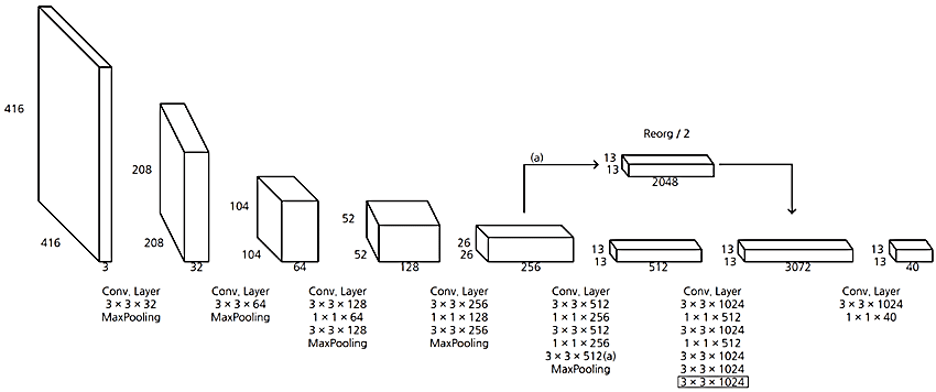
\includegraphics[width=0.9\linewidth]{datas/Darknet Framework.png}
    \caption{Darknet Framework, combination of 24 layers with 2 fully connected layers.}
    \label{fig:Darknet Framework}
\end{figure}

\begin{multicols}{2}
\subsection{YOLOv2}
Although YOLOv1 introduced object detection as a single regression problem, the limitations of this novel concept influenced the release of the new version - YOLOv2, also known as YOLO9000. The next stage of evolution was focused on improving existing weaknesses of the model, as well as improving accuracy without sacrificing the speed. Such upgrades led to the implementation of multiple features that are built on the foundation of YOLOv1. The new design of Darknet-19 architecture consists of 19 convolutional layers following 5 max-pooling layers. Reducing parameters by 60\%, while maintaining accuracy, which only required 5.58 billion operations to process an image. The bounding box prediction achieved better prediction results after incorporating anchor box prediction, a predefined set of boxes with different aspect ratios and scale. Instead of predicting the coordinates of each cell, the RPN predicts the offset of across the grid. Additionally, each convolutional layer adopted batch normalization technique, resulting in over 2\% improvement in mean Average Precision (mAP). YOLOv2 also makes effective use of the multi-scale method — a process of training the model on images at different scales to average the prediction, improving the detection of small objects.



\subsection{YOLOv3}
The third version of YOLO model proposed a new Darknet-59 backbone architecture which is made of 53 convolutional layers and incorporates residual blocks that vary from 3x3 to 1x1 layers (13x13, 26x26. 52x52). 

By integrating the Pyramid architecture, which closely resembles the Feature Pyramid Network (FPN), it effectively manages a feature map at three different resolutions, each of which is analyzed to produce a separate prediction grid. Thus, the model applies detection mechanisms more efficiently to objects of different sizes. Overall, YOLOv3 achieved better results compared to its precursor, which is deeper and more robust with improved data-loading performance.

\subsection{YOLOv4}
The release of YOLOv4 brought significant improvements to the architecture, shifting to a new CNN architecture named Cross Stage Partial Network (CSPNet), with the design of 54 layers, splitting the structure into three separate components: backbone, neck, and head, and each responsible for its own distinct feature, see \ref{fig:CSPNet}. The backbone employs convolutional neural networks to learn features throughout all layers. The neck part serves as a basis which is formed based on extracted features gathered across different layers. Finally, the head processes bounding box prediction, and works on class probabilities. One of the primary updates included in the fourth generation of the YOLO model revolves around the optimization, involving Mosaic Data Augmentation which combines 4 images rolled into one, increasing the number of contexts scenarios where object detection would work. Self-Adversarial Training (SAT) is designed to improve robustness and generalization, which makes the model think there is no object, with the double staged data augmentation approach. Cross-mini Batch Normalization (CmBN) optimizes the single GPU utilization during the training. Modified Spatial Attention Model (MSAM) helps the model focus on crucial features with no cost on the performance. 
\end{multicols}

\begin{figure}[ht]
    \centering
    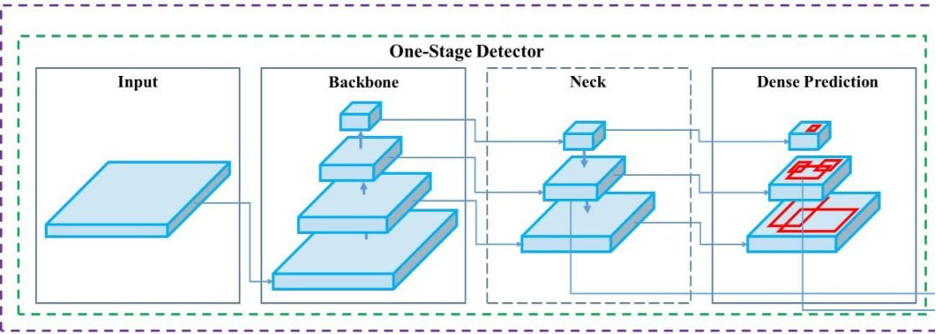
\includegraphics[width=1\linewidth]{datas/Cross Stage Partial Network (CSPNet).png}
    \caption{Cross Stage Partial Network (CSPNet), a 54 layered architecture with 3 separate components: Backbone, Neck and Head.}
    \label{fig:CSPNet}
\end{figure}
 
\begin{multicols}{2}
\subsection{YOLOv5}
Aiming for the better performance-wise benchmarks, an incremental advancement YOLOv5 was designed based on the previous version. Mainly, the developers focused on user-friendly aspects, simplifying model implementation and making the documentation more accessible by supporting multiple languages, and finally, the entire model was built on the PyTorch framework, making the technology more straightforward in application. 

Furthermore, transferring to a more complex architecture similar to the EfficientNet network framework called EfficientDet. The results of this change presents higher accuracy results, better generalization, and wider range of object categorization. Additionally, the new version presents a new pooling technique - Spatial Pyramid Pooling (SPP), which reduces the spatial scaling across the grid, which effectively detects objects of a smaller size. 


\subsection{YOLOv6}
The release of YOLOv6 has influenced application in the industrial sector, offering nicely tuned performance between speed and accuracy rate. Along with the architecture enhancement, the model incorporates Bi-directional Concatenation (BiC), Anchor-aided training (AAT) scheme, and the improved neck component. A newer version of architecture, EfficientNet-L2 required a smaller number of parameters, and received large processing power. The AAT strategy utilized an anchor-based method, accompanied by the anchor-free technique, which proposed a method that does not rely on a predefined set of anchor boxes with different resolutions, but only predicts the locations of center points and corner key points derived from the image features. Thus, expanding the capabilities of the detection mechanism. The BiC module is a part of the neck component that results in performance gains, by directly influencing the localization signals in the neck component. This iteration of YOLO has adopted several strategies to better optimize the computation of the model. For instance, during the training phase of the neural network, it assigns the labels to the predefined anchor boxes. Usually, this happens with the help of multiple strategies and of varying complexity. Including IoU method, ground-truth based technique, or SimOTA label assignment.

\subsection{YOLOv7}
Designers of YOLOv7 focused on refining the capabilities of previous versions, along with alternative technologies, demonstrating satisfying benchmarks. One of the major improvements is the increased FPS rates of the real-time image, achieving up to 155 frame per second processing. Making significant progress in the field of real-time detection, especially in time-sensitive scenarios such as autopiloting and surveillance. This generation of the model requires 50\% less computing load and decreases in the number of parameters as well by 40\%, achieving higher accuracy without an inference cost raise. In general, this version is considered as one of the fastest among leading alternatives in the field. By incorporating dynamic label assignments, extended and compound scaling and re-parameterization, it demonstrates satisfying benchmarks.

\subsection{YOLOv8}
YOLOv8 is one of the major and stable versions of the model, it involves advanced backbone and neck architecture. Offering a variety of pre-trained models where each designed for specific task, including object detection, instance segmentation, oriented object detection pose/keypoints detection and classification. In this generation, YOLOv8 avoided using an anchor-based approach, but instead took advantage of the anchor free method, relying on predicting the object centers. In terms of performance, it achieved cutting-edge results of 37.3 on the mAP score tested on COCO dataset with speed of 0.99ms using A100 TensorRT GPU. As of today, YOLOv8 remains widely used among many computer vision algorithms.

\subsection{YOLOv9}
The release of YOLOv9 marked a pivotal step in the deep neural network area, introducing highly effective solutions to the long-lasting challenges, by implementing a new innovative architecture called Generalized Efficient Layer Aggregation Network, or GELAN for short, and feature named - Programmable Gradient Information (PGI), incorporating these two essential enhancements, the model is able to address the issue data loss, improving the model retention and training capabilities. In the deep neural network, it is often the case when the data is passed deeper through the layers, but the more it goes on, the chances of information being lost increases. The application of PGI helps in avoiding by ensuring the integrity of the crucial data throughout all layers of the network. Compared to the previous generation, YOLOv9 demands even less computing and number of parameters, which are 25\% and 15\%, respectively. Generally, this generation of YOLO brings effective architecture design, improved accuracy and adaptability.

\subsection{YOLOv10}
YOLOv10 addressed the design flows of past YOLO iterations by becoming independent of post-processing tools such as non-maximum suppression (NMS) and refining the architectural structure to gain additional components, including a one-to-many head and a one-to-one head, in addition to the backbone and neck components that received upgrades as well. Better gradient flow, improved version of CSPNet, and decreased workload. The YOLOv10 takes advantage of the new key feature called dual assignment, employing both one-to-one and one-to-many techniques in the detection pipeline, where One-to-Many in the training phase, works with multiple predictions based on a single object and improves the learning curve. While One-to-One components reduce the latency by creating the prediction with the highest confidence score possible during the inference, resulting in efficiency gain. Together, these two modules make appropriate conditions to eliminate NMS technique.

\subsection{YOLOv11}
Currently, YOLOv11 remains one of the stable and commonly used versions in the family of YOLO models, being widely used in the industry and the community. Built over the last iterations of YOLOs, the 11th generation has achieved exceptional accuracy, speed and efficiency characteristics. Among the involved significant changes were the Enhanced Feature Extraction algorithm, redesign of architectural scheme, newer versions of feature pipelines, environment adaptability, and integrated wide range of varying tasks in the computer vision sector. The unique aspect of new architectural design is the implementation of components such as C3k2 Block and C2PSA Block minimizing the redundant computation and the number of parameters. C3k2 Block replaces the block of C2f block, dividing the structure of convolution into 2 convolutions but of a smaller scale. This approach showcased efficient wise boost compared to the CSP bottleneck. The purpose of C2PSA Block is to implement an attention mechanism that focuses around the most relevant regions across the image. Extracting the features on the smaller objects and within low-visible areas.
The model achieved cutting-edge performance metrics among the available models. 

In comparison, the 8th generation of YOLO, which is considered one of the stable versions among YOLO series, is outperformed by YOLOv11 in terms of feature extraction and processing metrics, being higher on mean Average Precision (mAP) using 22\% less parameters during the COCO dataset testing. Although both support versatile types of computer vision operations, but general accessibility of YOLOv11 makes a determining factor in choosing for this research, being environment-friendly system and requiring less parameters for testing

\subsection{YOLOv12}
At the time of writing, the YOLOv12 is the latest version available on February 18th, 2025. The major difference to the past generations of YOLOs, is the reconceptualized architecture of CNN, built over the years since YOLOv1. The novel approach in this architecture is an area attention mechanism, which splits the feature map into S equal sized areas. The idea is to avoid excessive complexity, reducing redundant workload. To address optimization challenges, Residual Efficient Layer Aggregation Networks (R-ELAN) was introduced as a novel method of feature aggregation, and block-level residual connections. As every model iteration, it improves over its predecessor in efficient utilization, accuracy, and performance load.

\end{multicols}
{\color{gray}\hrule}
\begin{center}
	\section{Applications And Impact}
	\textbf{How YOLO transforms research and practice in biomedicine and agriculture}
	\bigskip
\end{center}
{\color{gray}\hrule}
\begin{multicols}{2}
	The YOLO (You Only Look Once) object detection framework has proved remarkably adaptable across various fields, with especially promising uses in biomedical science and agriculture. This section examines how YOLO is applied in these domains, its actual and potential influence, and the obstacles that researchers and practitioners still need to overcome.

	\subsection{Biomedical Applications}
	\subsubsection{Cell Detection and Classification}
	YOLO's application for cell detection marks a notable advancement in biomedical imaging analysis \citep{ChanCell2020}. Traditional approaches to cell detection and counting often depend on time-consuming manual work, which tends to be both tedious and susceptible to human error. The speed and accuracy of YOLO offer a valuable alternative to these conventional methods.

	In both medical diagnostics and research contexts, where correctly identifying and categorizing cells is essential for testing and study, YOLO can reduce the burden of manual counting substantially \citep{electronics8030292}. This automation allows researchers and clinicians to process larger datasets more quickly, potentially speeding up discoveries and improving diagnostic results. The processing speed of YOLO—most evident in more recent versions such as YOLOv7, which can process up to 155 frames per second—makes it particularly useful for high-volume biomedical applications.

	Medical applications do, however, present specific challenges for object detection systems. Such applications require exceptional accuracy, particularly when working with small objects like individual cells in microscopic images \citep{ChanCell2020}. The ongoing development of YOLO through its various versions has gradually addressed these challenges, with better small object detection becoming a key focus in versions such as YOLOv3, which added a pyramid architecture to better handle feature maps at different scales \citep{redmon2018yolov3}.

	\subsubsection{Medical Imaging Analysis}
	Beyond cell detection, YOLO's impact extends to wider medical imaging applications. The system's ability to identify objects quickly and accurately makes it valuable for uses ranging from tumor detection to identifying anatomical structures in radiological images \citep{electronics8030292}. The more precise location capabilities in later YOLO versions, especially through improvements in bounding box prediction, allow for more accurate marking of areas of interest in medical images.

	The time-sensitive nature of many medical procedures makes YOLO's real-time processing especially valuable in clinical settings. For urgent diagnoses, the ability to analyze medical images quickly could improve patient outcomes by enabling faster medical interventions.

	\subsection{Agricultural Applications}
	\subsubsection{Fruit Ripeness Determination}
	In agriculture, YOLO's application for determining fruit ripeness addresses a key aspect of crop management \citep{Koirala2019}. Accurately assessing when fruits are ripe helps farmers decide the best harvesting times, which directly affects both produce quality and farming efficiency.

	Traditional ripeness assessment methods often rely on visual checks by farm workers, which can be inconsistent and subjective. By automating this process, YOLO offers the possibility of more objective and standardized ripeness evaluation \citep{KAMILARIS201870}. This has important implications for reducing food waste—a significant global issue—by ensuring that fruits are harvested at peak ripeness rather than too early or too late.

	The quality of agricultural produce relates directly to harvesting at the right stage of ripeness. YOLO's ability to accurately classify ripeness stages can help improve food quality, potentially allowing for better market prices and higher consumer satisfaction.

	\subsubsection{Challenges in Agricultural Implementation}
	Despite its potential, using YOLO in agricultural settings poses unique challenges. Unlike controlled laboratory environments, agricultural applications must cope with variable outdoor conditions, including changing light, complex backgrounds with vegetation, and different weather conditions \citep{KAMILARIS201870}.

	More recent YOLO versions have partly addressed these challenges. For example, YOLOv4 introduced Mosaic Data Augmentation, which combines multiple images to create diverse training scenarios, helping the model adapt better to different contexts—an important feature for agricultural applications where conditions rarely remain consistent \citep{bochkovskiy2020yolov4}. Similarly, YOLOv4's Self-Adversarial Training improves the model's resilience, potentially enhancing its performance in challenging agricultural environments.

	\subsection{Broader Impact}
	\subsubsection{Computational Efficiency and Accessibility}
	One of the most notable aspects of YOLO's evolution has been the steady improvement in computational efficiency \citep{Ultralytics2024}. Earlier object detection systems required substantial computing resources, limiting their practical use in resource-limited settings. The continued refinement of YOLO has addressed this limitation, with versions like YOLOv7 using 50\% less computing power and 40\% fewer parameters while achieving better accuracy.

	This improved efficiency has widened access to advanced object detection capabilities, making them available to more users and applications. For both biomedical and agricultural applications, this means that sophisticated image analysis can be used even in settings with limited computational resources, potentially extending these technologies to underserved areas.

	\subsubsection{Integration with Other Technologies}
	YOLO's impact goes beyond its standalone abilities \citep{8627998}. Its potential combination with other emerging technologies, such as Internet of Things (IoT) devices in agriculture or portable diagnostic tools in healthcare, creates new possibilities for real-time monitoring and analysis.

	For instance, in agriculture, YOLO could work with automated harvesting systems, allowing selective harvesting based on ripeness detection \citep{Koirala2019}. In biomedical applications, integration with point-of-care diagnostic devices could bring advanced cell detection capabilities to remote or resource-limited healthcare settings \citep{ChanCell2020}.
\end{multicols}
{\color{gray}\hrule}
\begin{center}
\section{Experimental Evaluation}
\textbf{Small description}
\bigskip
\end{center}
{\color{gray}\hrule}
\begin{multicols}{2}
\subsection{Subsection}
\lipsum[1]
\subsection{Subsection}
\lipsum[1-3]
\end{multicols}

{\color{gray}\hrule}
\begin{center}
\section{Advantages And Limitations}
\textbf{Small description}
\bigskip
\end{center}
{\color{gray}\hrule}
\begin{multicols}{2}
\subsection{Subsection}
\lipsum[1]
\end{multicols}

{\color{gray}\hrule}
\begin{center}
	\section{Future Directions And Conclusions}
	\bigskip
\end{center}
{\color{gray}\hrule}
\vspace{0.5cm}

This research examined YOLO's application in biomedical and agricultural fields, uncovering both significant capabilities and areas needing improvement. By testing YOLO v11 across COVID-19 X-ray analysis, blood cell detection, and fruit ripeness classification, we gained valuable insights into optimizing object detection models for specific domains.

\subsection{Current Performance and Evolution}

Our results show that YOLO's effectiveness varies substantially according to the application. In fruit ripeness detection, the near-perfect results (mAP@50: 0.995) demonstrate YOLO's strength with visually distinctive features. Blood cell detection showed strong results (mAP@50: 0.934), suggesting good potential for laboratory use, while COVID-19 X-ray analysis yielded more modest outcomes (mAP@50: 0.726), indicating that further refinement is necessary.

Interestingly, model size did not always predict performance. The smaller YOLOv11n model produced the best results for fruit ripeness detection, suggesting that for applications with clear visual differences, smaller models can be both effective and computationally efficient. This pattern matches broader trends in YOLO development, where design improvements often seek to balance detection accuracy with processing speed \citep{bochkovskiy2020yolov4}.

YOLO's evolution from earlier versions to current implementations reveals consistent improvements in both detection accuracy and computational efficiency. Studies comparing various models have repeatedly shown YOLO's advantages for real-time applications, with newer versions like YOLOv8 reaching accuracy rates of 0.998 on some datasets, far outperforming other models such as VGG16 \citep{Gunawan2024}. These improvements stem from architectural modifications that improve feature extraction while preserving YOLO's characteristic speed.

\subsection{Challenges and Limitations}

Our study contains several important limitations. The relatively small COVID-19 dataset likely limited model performance for that application. Also, while we examined two major industries, expanding to other fields would offer a more complete picture of YOLO's adaptability.

Beyond our research constraints, YOLO implementation faces wider challenges with data requirements and environmental variation. Data scarcity poses a basic constraint, especially for specialized applications where labeled examples are limited \citep{Mhalla2024}. Both the quality and diversity of training data affect model performance, and problems like class imbalance can introduce bias into trained models.

Environmental conditions present substantial challenges for real-world use. Changes in lighting, weather, and background complexity can significantly affect detection performance, particularly in outdoor settings \citep{Akbar2024, Tsitos2024}. Models trained under specific conditions often perform worse when used in different environments. Additionally, high-performance object detection models may require more computational resources than available on edge devices where real-time processing is needed \citep{Kumar2024}.

\subsection{Future Research Directions}

Based on our findings and current trends in YOLO development, we suggest several promising research paths:

\subsubsection{Enhanced Medical Image Processing}
Future work should aim to improve YOLO's detection of subtle patterns in medical images. This might include creating specialized preprocessing techniques similar to our R-LBP method but designed specifically for radiological images. Exploring mechanisms that direct attention to important regions in medical scans could also prove useful, as recent research into transformer-based models for visual analysis suggests \citep{Gunawan2024}.

\subsubsection{Small Object Detection Improvement}
The difficulty of detecting small, overlapping objects (particularly evident in blood cell detection) deserves further study. Creating YOLO variants with better feature extraction at smaller scales could address this weakness, possibly through modified anchor box approaches or techniques that combine features across different resolutions.

\subsubsection{Architectural Modifications}
Research indicates that adding attention mechanisms like those in transformer-based models might improve future YOLO development \citep{Gunawan2024}. These mechanisms would help YOLO focus on relevant image features while ignoring unimportant information, potentially addressing current limitations in analyzing complex scenes. Additionally, combined approaches that merge YOLO's speed with other models' strengths show promise, as seen in UNet-based YOLO approaches for challenging visual environments \citep{Zukal2024}.

\subsubsection{Computational Efficiency}
As applications increasingly require deployment on devices with limited resources, research into model compression, quantization, and hardware-specific optimizations will become more important \citep{Espinoza2023}. These developments should maintain detection performance while reducing model size and computational needs, allowing broader use across various hardware platforms. Future YOLO versions might include methods that adjust processing complexity based on image content, allowing better resource use during operation \citep{Kumar2024}.

\subsubsection{Integration with Other Technologies}
Combining YOLO with other technological approaches represents an important area for future development. Multi-modal integration, merging visual data with other sensor inputs like infrared, LIDAR, or audio, could greatly improve detection capabilities in difficult environments \citep{Espinoza2023}. This approach would allow YOLO models to use complementary information sources, potentially overcoming limitations of purely visual analysis in conditions with poor lighting, occlusion, or bad weather.

\subsubsection{Cross-Domain Transfer Learning}
Studying how knowledge gained in one field (e.g., agricultural object detection) might transfer to another (e.g., medical imaging) could create more data-efficient training methods. This is especially relevant for medical applications where annotated data is often limited. Transfer learning and knowledge distillation techniques could enable more efficient training and better generalization across domains, allowing models trained on one type of object to more effectively detect similar objects in different contexts \citep{Mhalla2024}.

\subsection{Practical Implications}

Our research offers several practical guidelines for implementing YOLO across different domains:

For agricultural applications, the lightweight YOLOv11n model offers an excellent balance of accuracy and efficiency, making it appropriate for field conditions or embedded systems. The R-LBP preprocessing technique we developed appears particularly useful for enhancing texture-based classification tasks.

For biomedical applications, the choice of model variants depends on the specific task. Blood cell detection works better with larger models (YOLOv11l) and longer training periods, while COVID-19 detection might need domain-specific data augmentation strategies to improve performance with limited datasets.

The real-time capabilities shown across all applications (33-200 FPS) highlight YOLO's value for time-sensitive tasks in both domains. This performance enables applications like automated sorting systems in agriculture and quick screening tools in healthcare.

\subsection{Impact Across Domains}

YOLO's impact extends well beyond our specific research focus. In agricultural applications, YOLO-based systems have achieved impressive results in disease detection, such as 97.56\% precision in identifying Wheat Streak Mosaic Virus \citep{Akbar2024}. These capabilities allow automated quality control, yield estimation, and harvest optimization that were previously impractical due to labor requirements.

In safety and security applications, YOLO models have shown considerable value for personnel protection and accident prevention. Studies comparing YOLOv5n and YOLOv8n models for safety equipment detection on construction sites demonstrate these approaches can monitor personal protective equipment compliance in hazardous environments \citep{Karasu2024}.

Environmental protection efforts have benefited from YOLO implementations, particularly for wildfire detection and wildlife conservation. Research on wildfire and smoke detection using YOLO-NAS showed excellent performance, achieving over 91\% mAP@0.50 on webcam and infrared datasets \citep{Tsitos2024}. This capability allows early detection of fire events, potentially before they grow into uncontrollable wildfires.

Infrastructure maintenance has improved through YOLO applications in defect detection, especially for road conditions. Studies of real-time pothole detection systems using deep learning techniques show how YOLO-based approaches allow automated road condition monitoring that works more efficiently and consistently than traditional manual inspection methods \citep{Kumar2024}.

\subsection{Concluding Remarks}

YOLO has shown remarkable adaptability across biomedical and agricultural domains, with performance that varies predictably based on task characteristics. The model's adaptability to different applications through domain-specific modifications represents a significant advantage for researchers and practitioners seeking efficient object detection solutions.

Looking ahead, we expect that continued improvements in YOLO architecture, along with domain-specific adaptations like those we explored, will further extend the model's usefulness. As object detection technology advances, the gap between research and real-world implementation will narrow, bringing benefits to healthcare, agriculture, and potentially many other fields.

The path to widespread adoption will require addressing the limitations identified in this study, particularly for challenging cases like subtle medical abnormalities or small, overlapping objects. However, the rapid pace of development in computer vision suggests that many of these challenges may soon be overcome, opening new possibilities for automation and analysis across diverse domains.
\bibliographystyle{apalike}
\bibliography{references}
\end{document}
